\chapter{Anexo}

    \section{Problemas y Ejercicios}
        En esta sección se aborda la solución de los problemas solicitados durante las clases previas a la práctica. 

        \subsection{Ejercicio 1}
            \textit{Descripción}: Contestar las siguientes preguntas.

            \begin{enumerate}
                \item Documentar el orden de complejidad de la mochila fraccionaria.
                \textbf{Respuesta:} El orden de complejidad de la mochila fraccionaria es \(\theta(n\log{n})\)
                \item Mostrar mediante un contraejemplo que en el caso de elegir objetos enteros, el algoritmo voraz propuesta para el caso fraccionario puede no generar soluciones óptimas.
                \textbf{Respuesta:} No funcionaría por el simple hecho de que un objeto entero no puede generar una solución de un valor entero. 
                \item ¿Cuál sería la mejor función de selección voraz en el caso en el que todos los objetos tuvieran el mismo valor?
                \textbf{Respuesta:} Se basaría en los valores más pequeños, al ser todos iguales algunos se queden fuera si la mochila queda sin espacio.
                \item ¿Cuál sería la mejor función de selección voraz en el caso en el que todos los objetos tuvieran el mismo peso?
                \textbf{Respuesta:} No afectaría ya que se mira por el valor y no por el peso. 
                
            \end{enumerate}
            
            

            

        \newpage
        \subsection{Ejercicio 2}
            \textit{Descripción}: Construir la codificación de Huffman para la cadena ciencias de la tierra.
            \newline
            En la figura \ref{fig:huffman1} se muestra el árbol construido por medio de una página web de la cadena Ciencias de la Tierra.
            \begin{figure}[htp!]
                \centering
                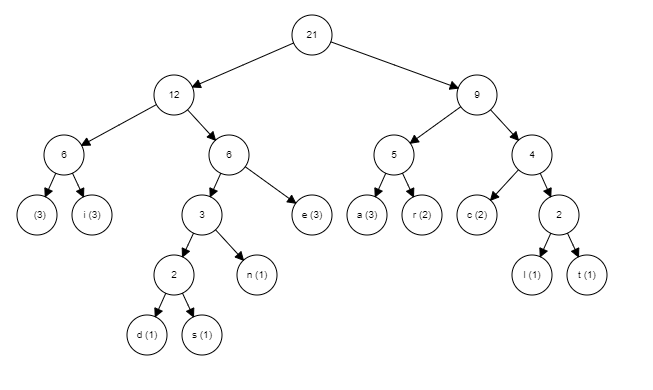
\includegraphics[width=0.7 \textwidth]{Images/HUFFMAN/HUFFMAN_CT.png}  
                \caption{Codificación cadena Ciencias de la Tierra}
                \label{fig:huffman1}
            \end{figure}
    
                
        \subsection{Ejercicio 3}
            \textit{Descripción}: Determinar el orden de complejidad el algoritmo de Huffman
            \newline
            La extracción de una cola de prioridad y al ser iterativo tiene una complejidad de \(O = n\log{n}\) 
            

        \subsection{Ejercicio 4}
            \textit{Descripción}: Documentar el orden de complejidad del algoritmo de Kruskal
            \newline
            Tiene una complejidad de \(O = n\log{n}\) Siendo n el número de vértices y a el número de aristas del grafo. Éste orden de complejidad es el obtenido al realizar la ordenación de las aristas de menor a mayor peso \cite{Kruskal}.
            
        \subsection{Ejercicio 5}
            \textit{Descripción}: Investigar el algoritmo de Prim
            \newline
            El algoritmo de Prim, dado un grafo conexo, no dirigido y ponderado, encuentra un árbol de expansión mínima. Es decir, es capaz de encontrar un subconjunto de las aristas que formen un árbol que incluya todos los vértices del grafo inicial, donde el peso total de las aristas del árbol es el mínimo posible.
            Después de realizar el análisis del código, tal y como muestran los costes indicados en el apartado anterior, se puede decir que, para el algoritmo de Prim, el orden de complejidad computacional temporal es de \(O(n^{2})\)). Siendo n el número de vértices del grafo \cite{Prim}.
                
        \subsection{Ejercicio 6}
            \textit{Descripción}: Documentar el orden de complejidad del algoritmo de Dijkstra.
            \newline
            El algoritmo de Dijkstra es un algoritmo eficiente de complejidad de \(O(n^{2})\) que sirve para encontrar el camino de coste mínimo desde un nodo origen a todos los demás nodos del grafo.
            